% lecture notes by Umut Özer
% course: gr
\lhead{Lecture 15: November 15}
\begin{claim}
  In fact, de Sitter spacetime can be embedded in five-dimensional Minkowski space, which is $\mathbb{M}^5 = (\mathbb{R}^{1, 4}, g)$ with metric
  \begin{equation}
    \label{eq:15-hash}
    ds^2 = -(dX^0)^2 + \sum_{i=1}^{4} (dX^{i})^2
  \end{equation}
  as the surface $-(X^0)^2 + \sum_{i=1}^{4} (X^{i})^2 = R^2$.
  The metric gets pulled back onto this surface.
\end{claim}
\begin{proof}
  Let $r^2 = \sum_{i=1}^{3} (X^{i})^2$ and $X^0 = \sqrt{R^2 - r^2} \sinh(t/R)$, $X^4 = \sqrt{R^2 - r^2} \cosh(t/R)$. In particular, this means that $(X^4)^2 - (X^0)^2 = R^2 - r^2$.
  \begin{exercise}
    You can check that if you compute $dX^0 = f dR + g dt$ and $dX^4 = \dots$, and plug these into the Minkowski spacetime metric \eqref{eq:15-hash}, you recover the de Sitter metric.
  \end{exercise}
\end{proof}
These coordinates are not particularly symmetric, meaning that $X^4$ has been singled out from $X^{1, 2, 3}$, and, moreover, cover only $X^4 \geq 0$.
A better choice of coordinates is
\begin{equation}
  X^0 = R\sinh( \frac{\tau}{R}) \quad \text{ and } \quad X^{i} = R \cosh( \frac{\tau}{R}) y^{i},
\end{equation}
where $y^{i}$ parametrise a 3-sphere, i.e.~$\sum_{i = 1}^{4} (y^{i})^2 = 1$.
These are called \emph{global coordinates} on \texttt{dS}.
\begin{exercise}
  Another small calculation you can do is to look at the variation again and plug it into \eqref{eq:15-hash} to give
  \begin{equation}
    ds^2 = -d\tau^2 + R^2 \cosh^2\left(\frac{\tau}{R}\right) d\Omega^2_3,
  \end{equation}
  where $d\Omega_3^2$ is the metric on $S^3$.
  This is called the \emph{FRW} form of the metric.
\end{exercise}
We know that this metric must also solve the Einstein equation with the same cosmological constant (as it must!), since there is a coordinate transformation that takes us from de Sitter (\texttt{dS}) spacetime to this; they describe the same spacetime.
This form of the metric has a natural cosmological interpretation in terms of an initially contracting and later expanding universe.
For the past three billion years or so, this has been a fairly good approximation to our universe.
\begin{leftbar}
  \begin{remark}
    Note that the first metric is the one that de Sitter found very soon after Einstein's theory was published.
    He found that immoving two observers move away from each other, and also calculated the redshift that emerged when those two observers sent light rays between each other.
    In particular, the first observations of Hubble and Slipher of the redshift were called the de Sitter effect.
    However, Hubble never believed in the expanding universe, which everyone credited him with, because the first metric seems to be independent of time.
    The second metric is more closely related to our notion of time, in which the universe actually (first contracts and then) expands with increasing $\tau$.
  \end{remark}
\end{leftbar}

\subsection{\texorpdfstring{$\Lambda < 0$}{Negative Cosmological Constant}: Anti-de Sitter Spacetime}%
\label{sub:anti_de_sitter_spacetime}

Let us look at some more solutions to the Einstein equations. Specifically, let us consider a negative cosmological constant $\Lambda < 0$. Again, we look for solutions of the kind
\begin{equation}
  ds^2 = -f(r)^2 dt^2 + f(r)^{-2} dr^2 + r^2 d\Omega^2_2.
\end{equation}
Exactly the same calculation as before gives us $f(r) = \sqrt{1 + r^2/R^2}$ with $R^2 = -3/\Lambda$.
This is \emph{anti-de Sitter} (\texttt{AdS}) spacetime. The plus sign rather than minus sign means that there is no coordinate singularity.
Repeating the geodesic calculations, we find that this time, massive geodesics obey $\dot{r}^2 + V_{\text{eff}}(r) = E^2$ (designed to look like Newtonian mechanics) with $V_{\text{eff}}(r) = (1 + l^2/r^2) (1 + r^2/R^2)$.
$l$ is to be interpreted as angular momentum.
This is illustrated in \ref{fig:angmombar2}.
\begin{figure}[htpb]
  \centering
  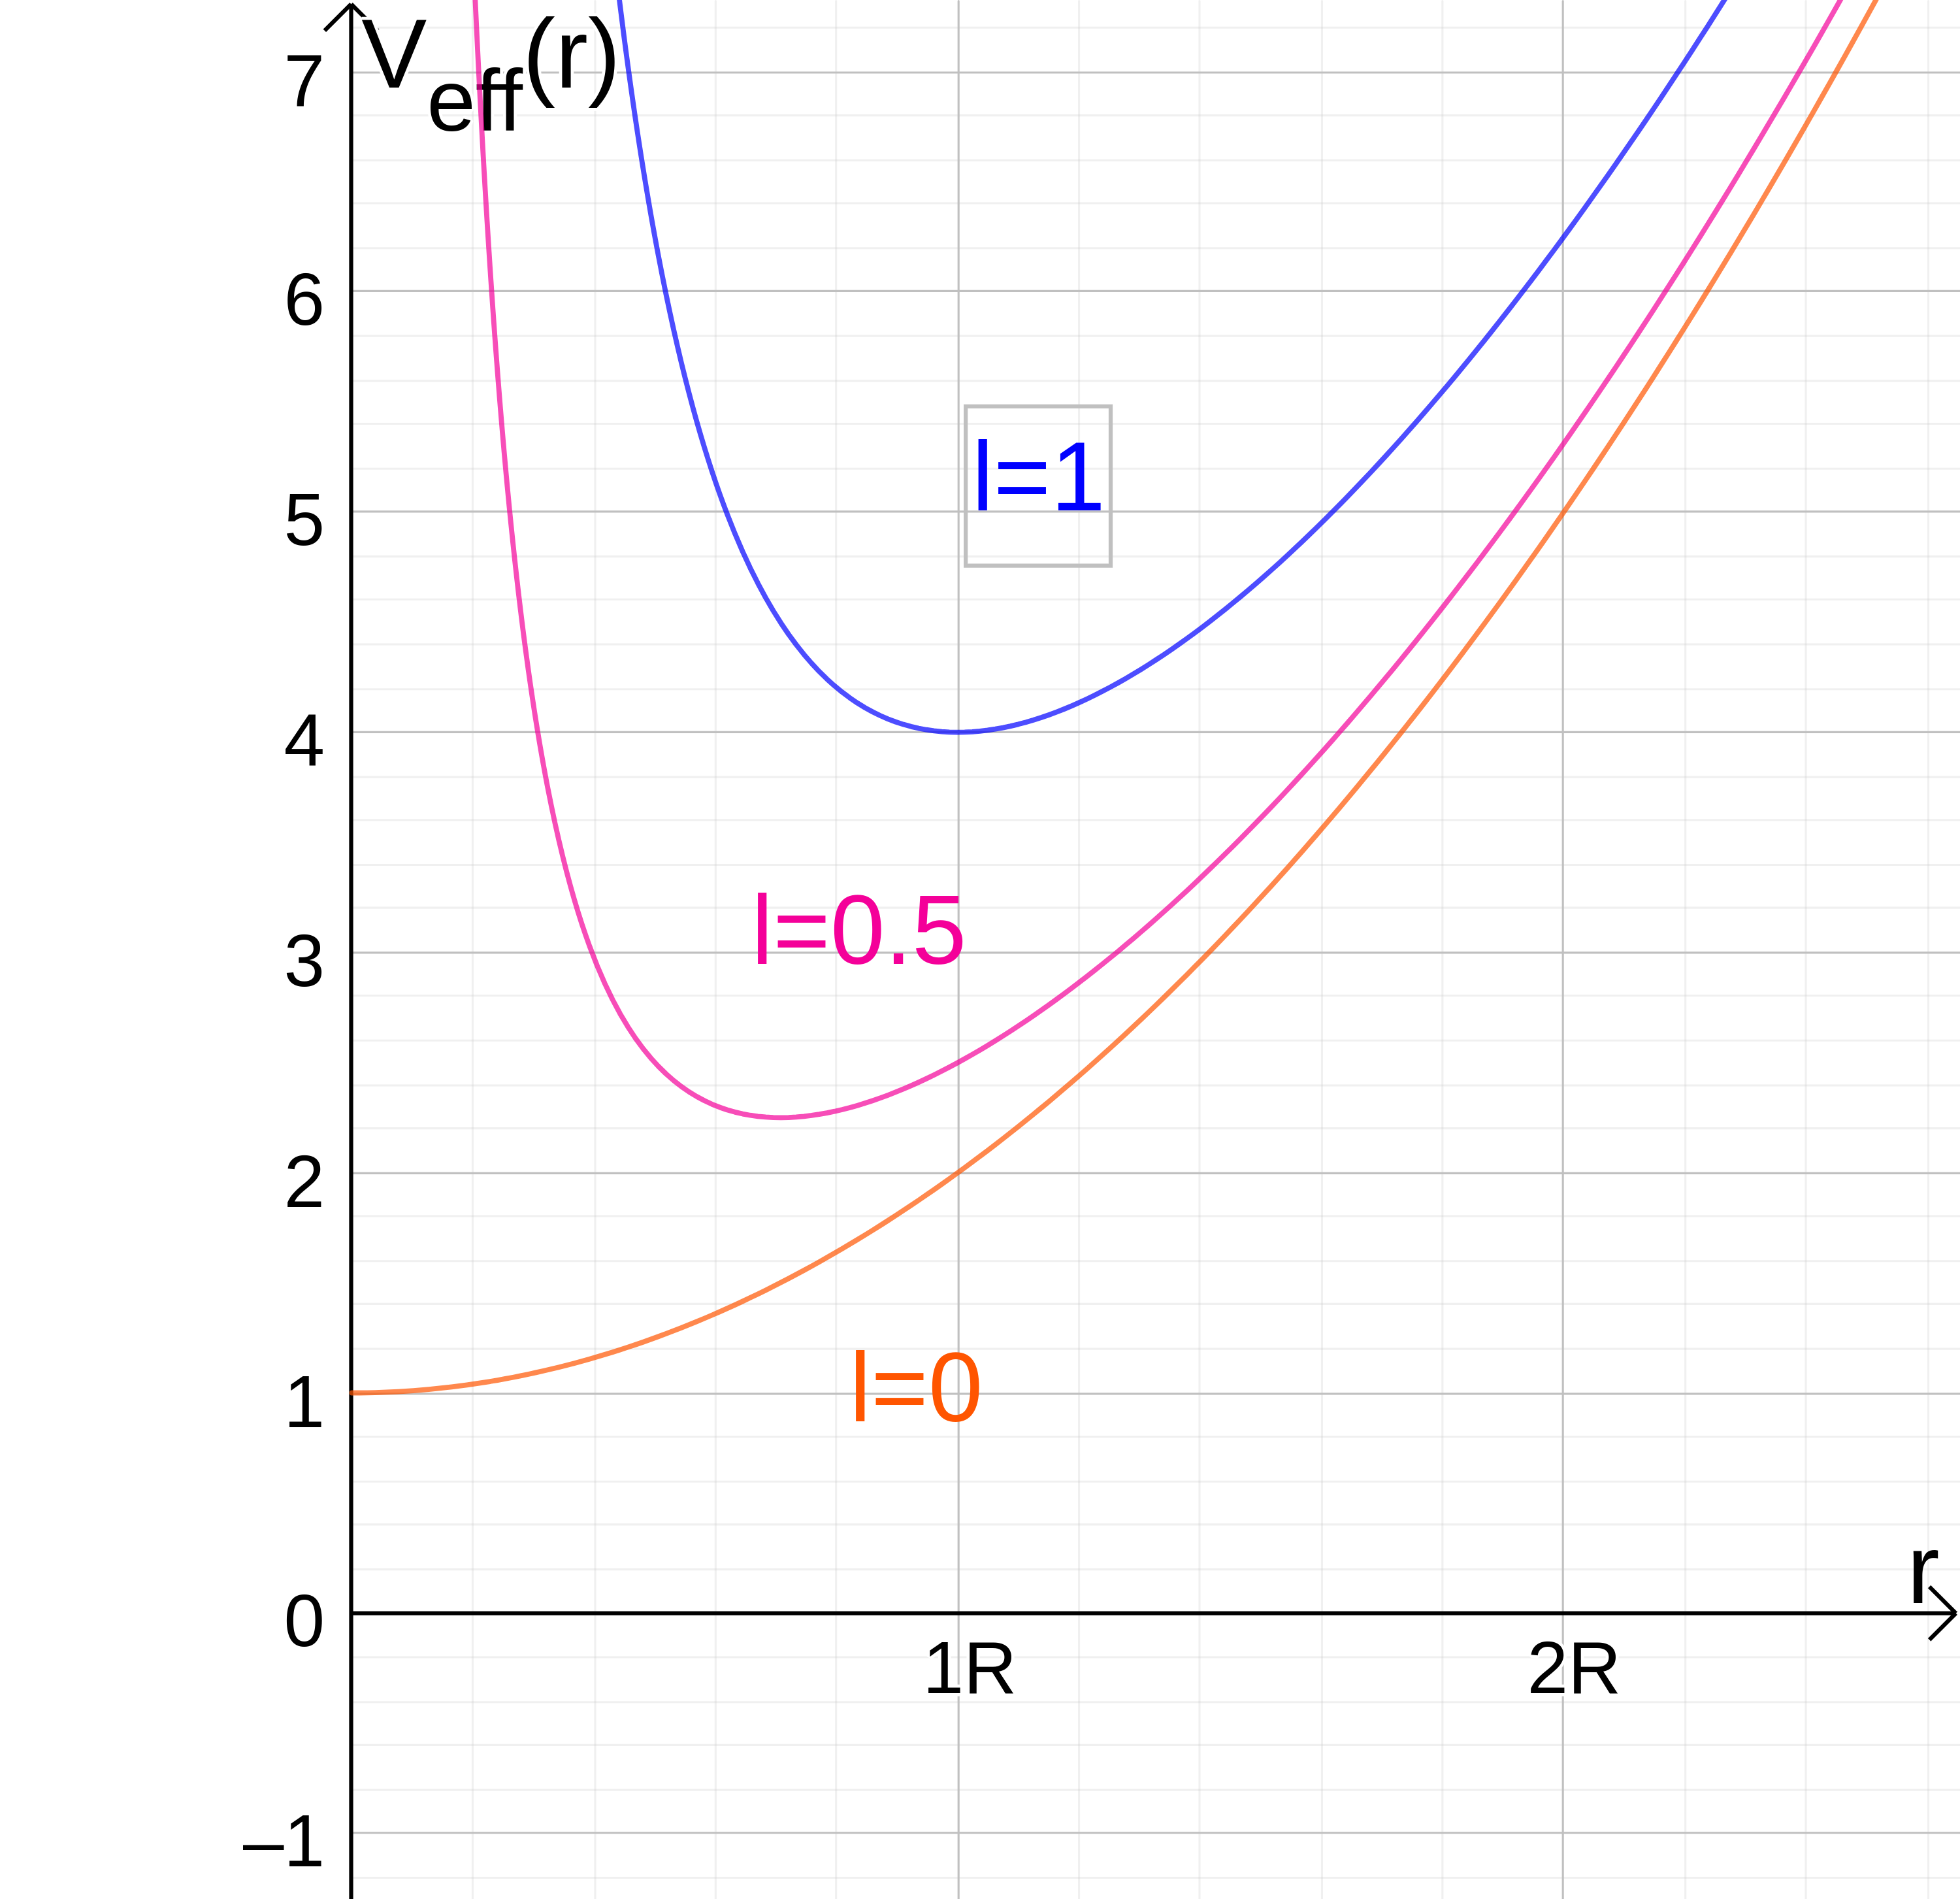
\includegraphics[width=0.5\linewidth]{angmombar2}
  \caption{}
  \label{fig:angmombar2}
\end{figure}
In particular, massive particles are confined to the centre of \texttt{AdS}.
With a finite amount of energy, there is only so far we can get before we fall back towards low $r$.
Massless particles follow null geodesics 
\begin{equation}
  -f^2 \dot{t}r^2 + f^{-2} \dot{r}^2 + r^2(\dot{\theta}^2 + \sin^2\theta \dot{\phi}^2) = 0.
\end{equation}
The right hand side is now zero.
At $\theta = \pi/2$, $\dot{\theta} = 0$, we have 
\begin{equation}
  \label{eq:null-15}
  \dot{r}^2 + V_{\text{null}}(r) = E^2 \qquad
  V_{\text{null}} = \frac{l^2}{2r^2} \qty(1 + \frac{r^2}{R^2}).
\end{equation}
This qualitatively changes the behaviour of the potential, as illustrated in Figure \ref{fig:angmombar3}.
\begin{figure}[htpb]
  \centering
  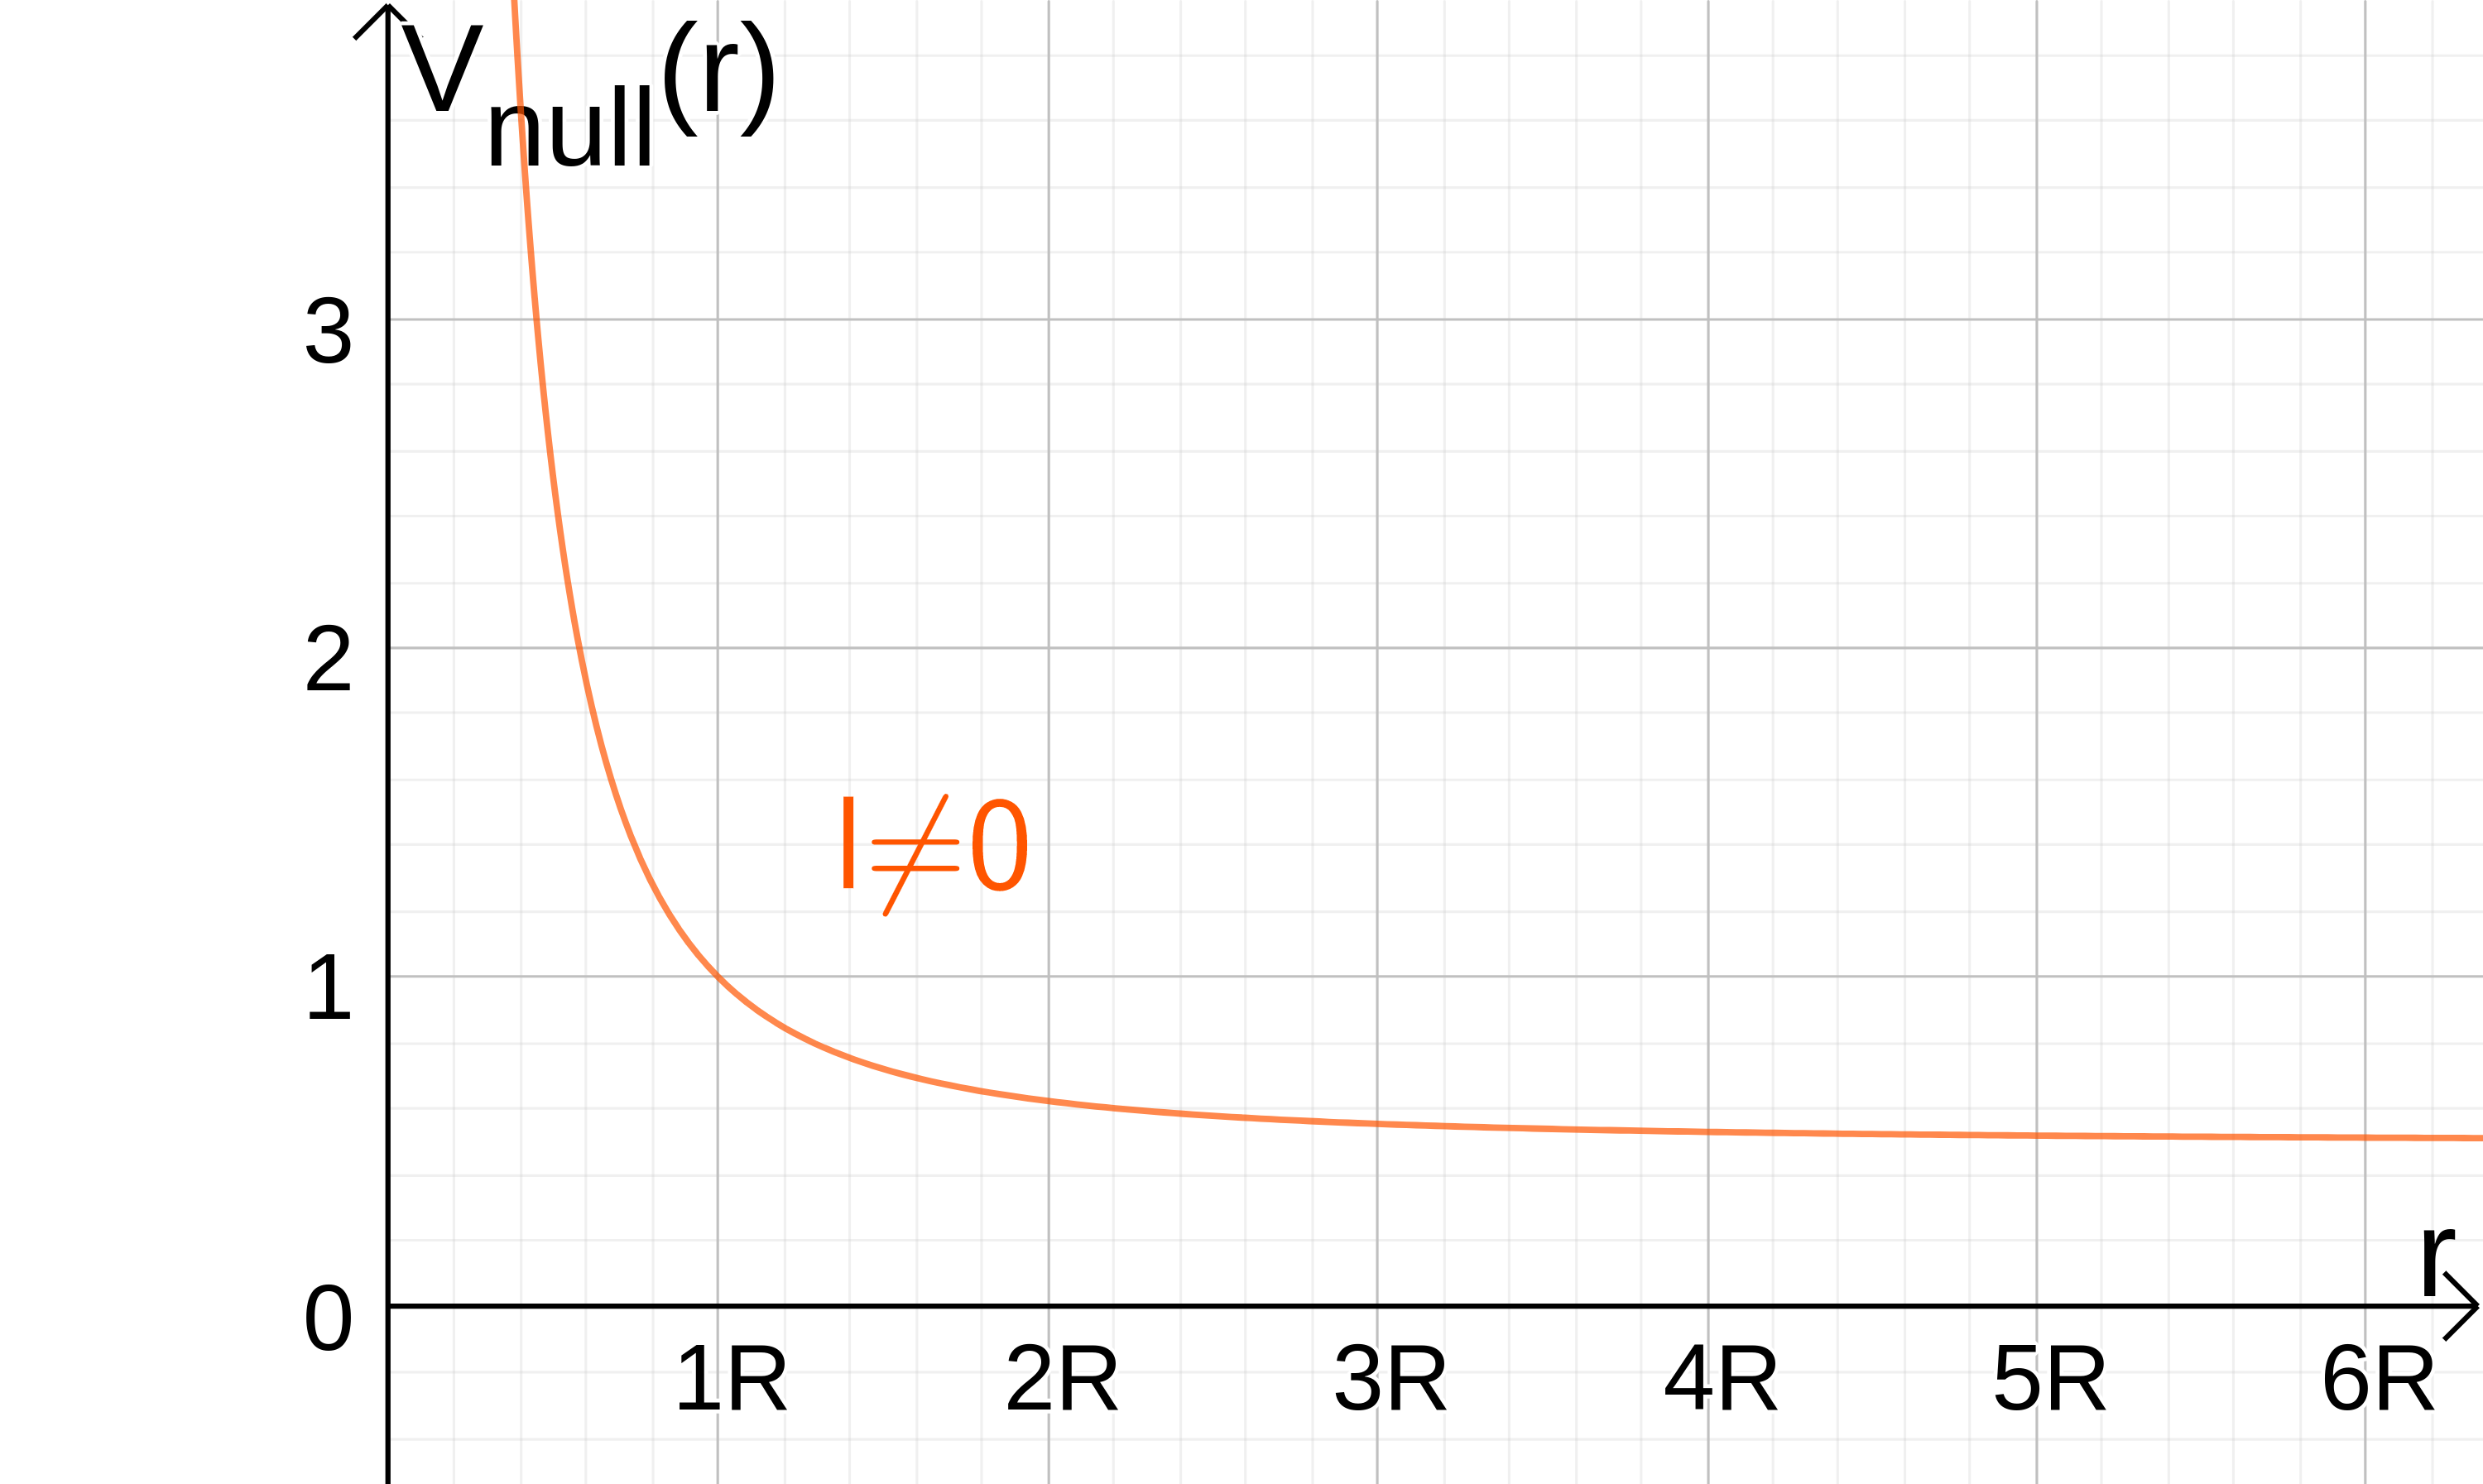
\includegraphics[width=0.5\linewidth]{angmombar3}
  \caption{}
  \label{fig:angmombar3}
\end{figure}
There is nothing that stops the light rays to go as far as they like to $r \to \infty$.

Introduce new coordinates $r = R\sinh \rho$. The \texttt{AdS} metric becomes
\begin{equation}
  \label{eq:15-AdS-new}
  ds^2 = -\cosh^2\rho \, dt^2 + R^2 \left[ d\rho^2 + \sinh^2\rho \, d\Omega_2^2 \right].
\end{equation}
The $\sinh$ is chosen to simplify the radial coordinate.
The null geodesic equation \eqref{eq:null-15} is
\begin{equation}
  R \dot{\rho} = \pm \frac{E}{\cosh\rho} \quad\implies\quad R \sinh\rho = E (\sigma - \sigma_0),
\end{equation}
where $\sigma$ is an affine parameter.
Massless particles hit $\rho \to \infty$ as $\sigma \to \infty$.
However, going back to $E = \cosh^2\rho \dot{t}$, the equation which defines the energy, we have $R \tan(t/R) = E (\sigma - \sigma_0)$.
So $t \to \frac{\pi R}{2}$ as $\sigma \to \infty$. Massless particles reach infinity of \texttt{AdS} in finite coordinate time.
\begin{claim}
  Like \texttt{dS}, \texttt{AdS} can be viewed as a hyperboloid in $\mathbb{R}^{2, 3}$
  \begin{equation}
    -(X^0)^2 - (X^4)^2 + \sum_{i=1}^{3}(X^{i})^2 = R^2.
  \end{equation}
\end{claim}
\begin{proof}
  To see this, let
  \begin{subequations}
    \begin{align}
      X^0 &= R \cosh \rho \sin(\frac{t}{R}) \\
      X^4 &= R \cosh \rho \cos(\frac{t}{R}) \\
      X^{i} &= R y^{i} \sinh\rho,
    \end{align}
  \end{subequations}
  where $\sum_{}^{} (y^{i})^2 = 1$ defines a two-sphere and we recover the \texttt{AdS} metric in the form \eqref{eq:15-AdS-new}. 
\end{proof}
There is one last set of coordinates, which \texttt{AdS} is most often written in in the physics literature:
\begin{subequations}
  \begin{align}
    X^{i} &= \frac{\widetilde{r}}{R} x^{i}, \qquad i = 0,1,2   \\
    X^4 - X^3 &= \widetilde{r} \\
    X^4 + X^3 &= \frac{R^2}{\widetilde{r}} + \frac{\widetilde{r}}{R^2} \eta_{ij} x^{i} x^{j}
  \end{align}
\end{subequations}
Computing the metric from this parametrisation gives
\begin{equation}
  ds^2 = R^2 \frac{d\widetilde{r}^2}{\widetilde{r}^2} + \frac{\widetilde{r}^2}{R^2} + \frac{\widetilde{r}^2}{R^2} \eta_{ij} dx^{i} dx^{j}.
\end{equation}
This is called the \emph{Poincar\'e patch}. It does not cover the whole of \texttt{AdS}. 
Unlike \texttt{dS} spacetime, \texttt{AdS} is not connected to our universe (as far as we can tell); however, it is an important spacetime in which we understand the behaviour of quantum gravity, which makes it worth studying!
